\section{Design}


\subsection{Overordnet System Design}
\noindent Dette afsnit repræsenterer hvordan modulerne ønskes at kommunikere med hinanden samt give et overblik over hvor meget der kommunikeres mellem modulerne i de forskellige stadier. Der vil i dette afsnit indgå 4 User stories til at repræsentere systemets design. Disse User Stories er relevante for design, da de involverer alle moduler samtidigt og giver et indblik i kommunikationen på tværs af systemet.

\noindent Herunder ses et sekvensdiagram for User Story 7-10 - Save. Her ses hvordan det ønskes at de forskellige moduler kommunikerer på tværs af systemet når en bruger loader et save fra databasen.
\begin{figure}[H]
\centering
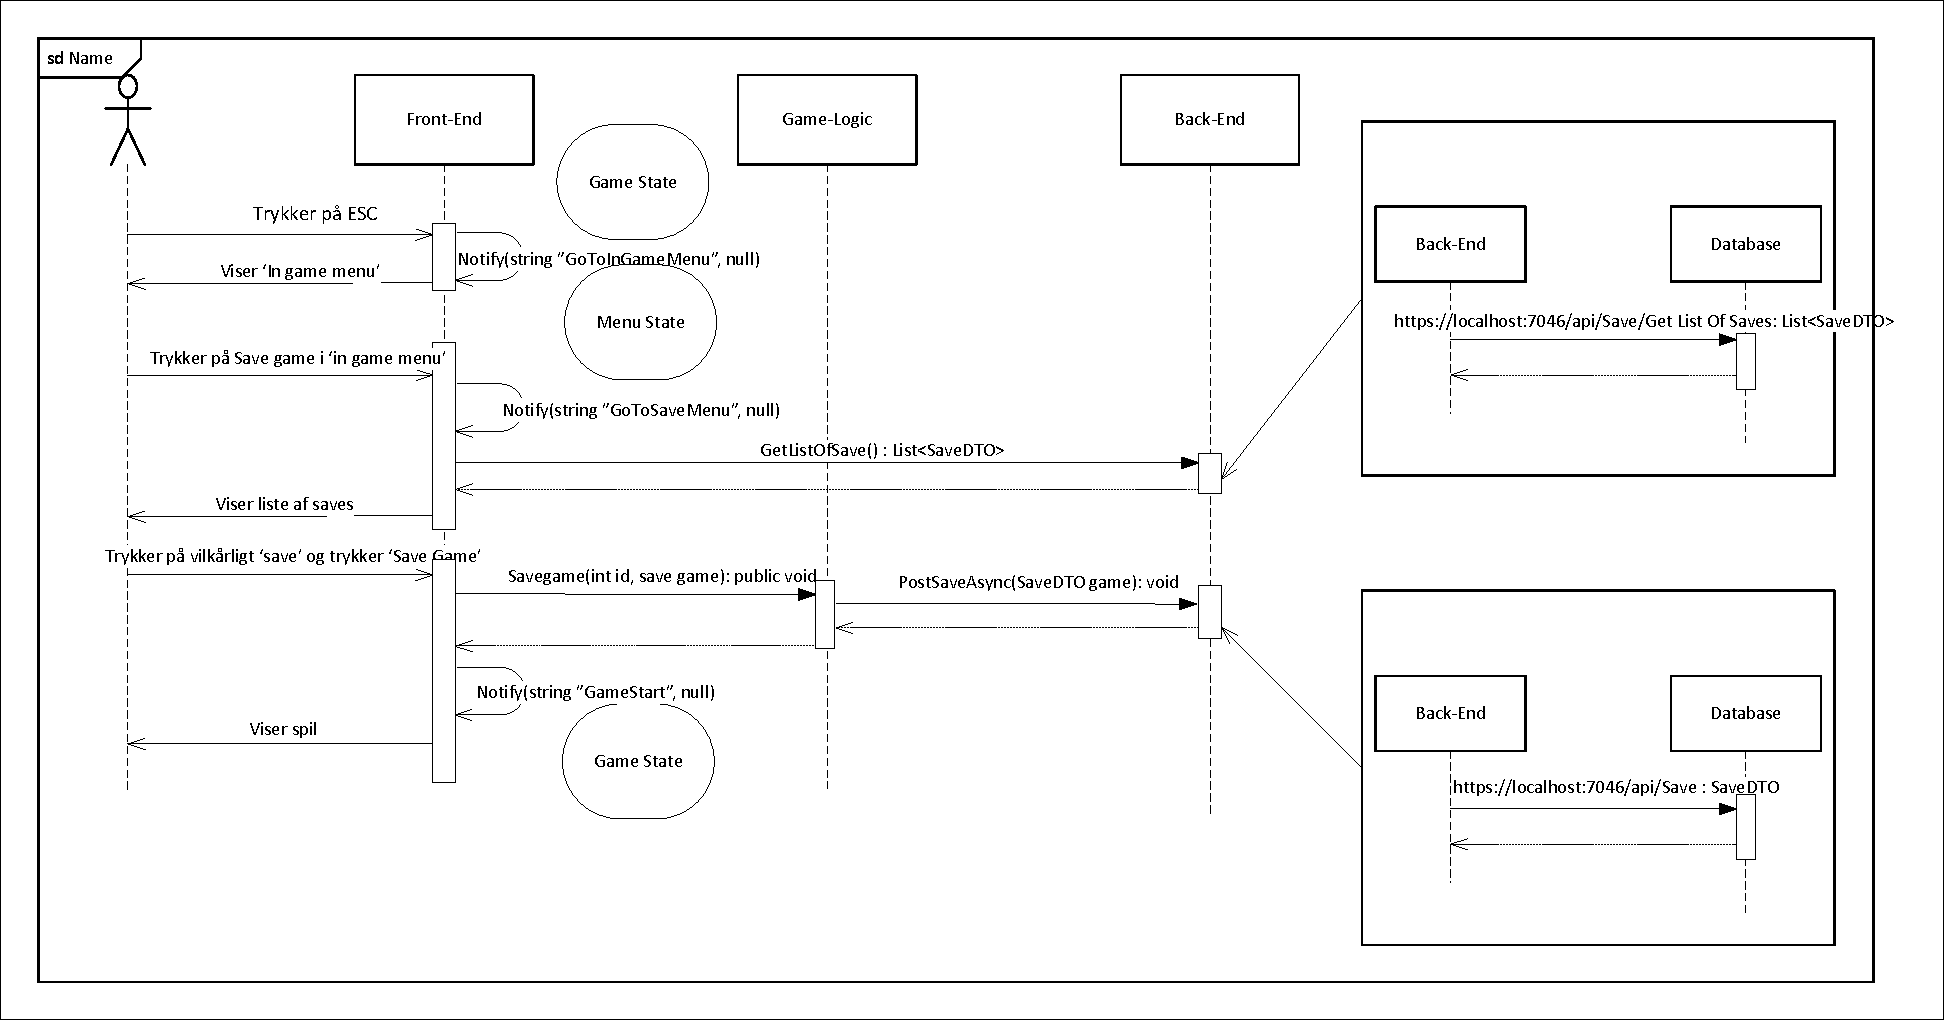
\includegraphics[width = \textwidth]{02-Body/Images/Arkitektur - SD Save Game}
\caption{SD diagram for User Story 7-10. Diagrammet viser hvordan det ønskes at systemet overordnet skal kommunikere på tværs af hinanden når en bruger skal gemme sit aktuelle save}
\label{fig:Arkitektur-SD-SaveGame}
\end{figure}

\noindent Herunder ses et sekvensdiagram for User Story 17-18 - Load. Her ses hvordan det ønskes at de forskellige moduler kommunikerer på tværs af systemet når bruger gemme et save i databasen.
\begin{figure}[H]
\centering
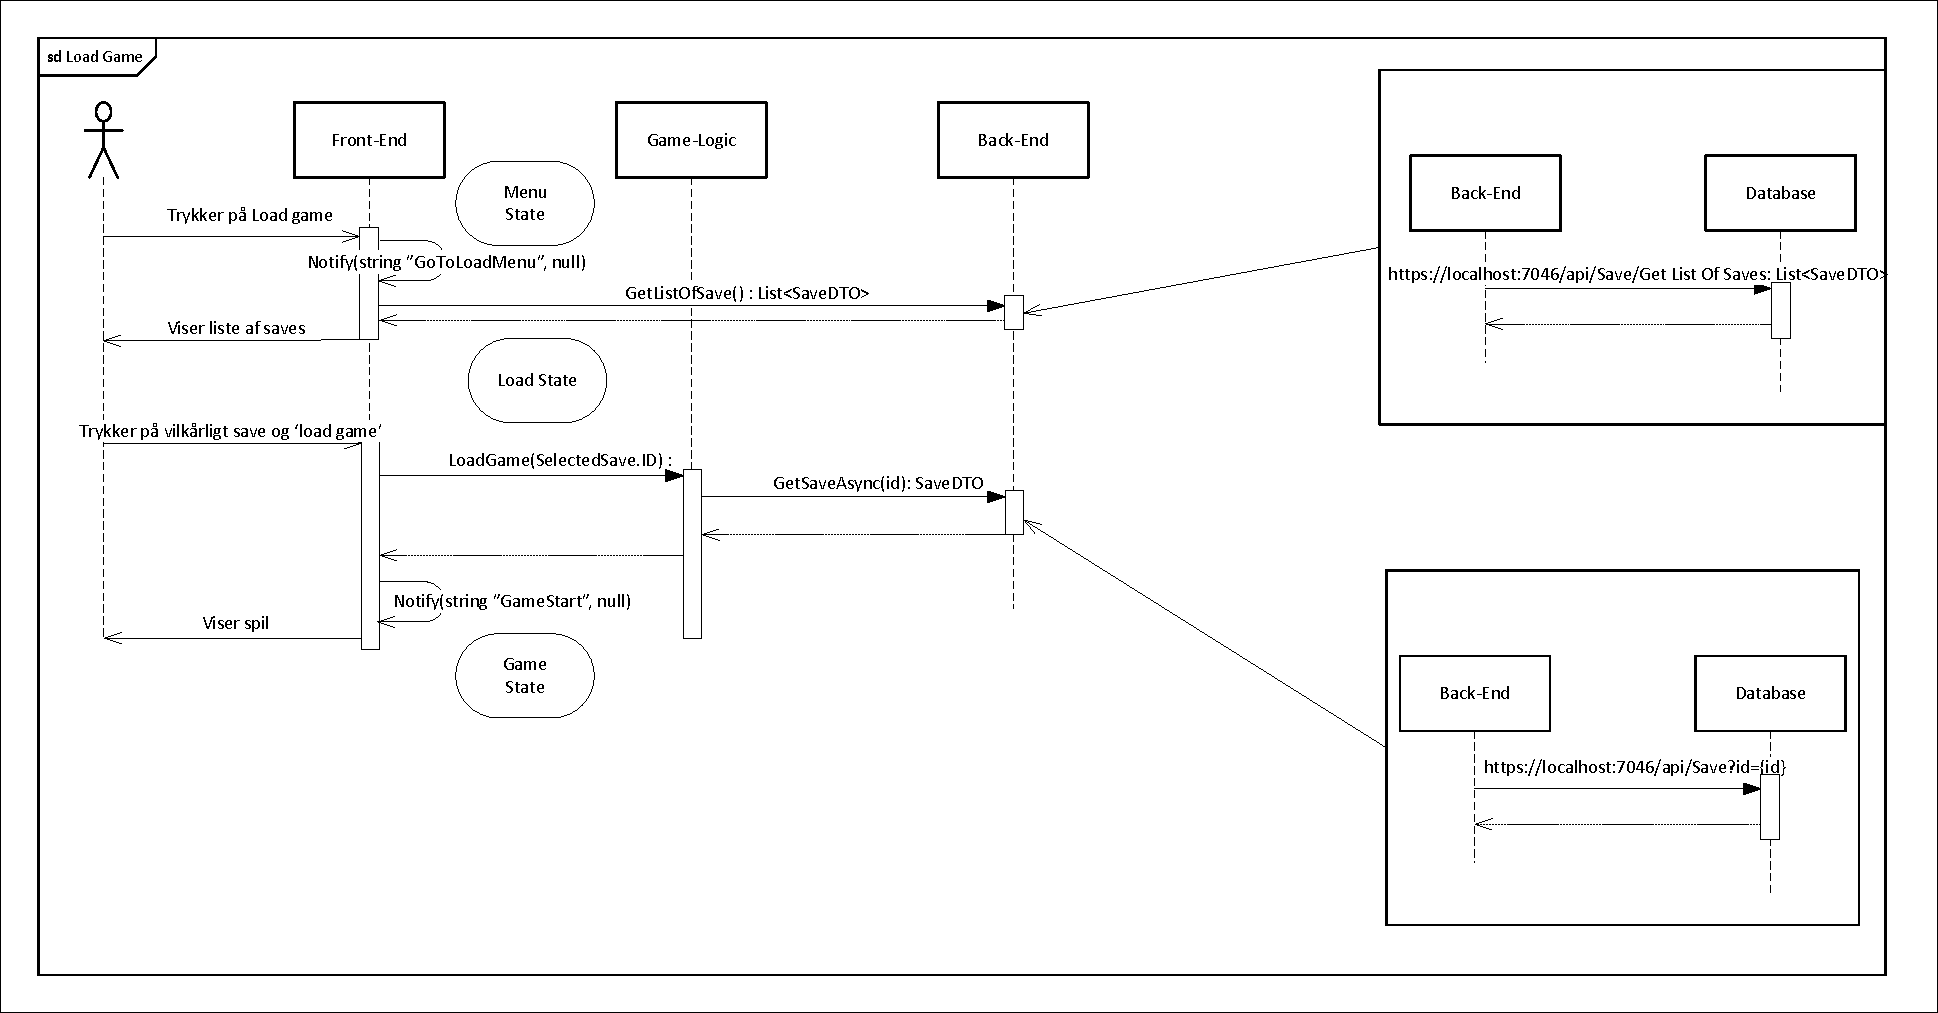
\includegraphics[width = \textwidth]{02-Body/Images/Arkitektur - SD Load Game}
\caption{SD diagram for User Story 17-18. Diagrammet viser hvordan systemet overordnet skal kommunikere på tværs når bruger skal loade sit aktuelle save. }
\label{fig:Arkitektur-SD-LoadGame}
\end{figure}

\noindent Herunder ses et sekvensdiagram for User Story 1 - Log in. Her ses hvordan det ønskes at de forskellige moduler kommunikerer på tværs af systemet når bruger skal logge ind.
\begin{figure}[H]
\centering
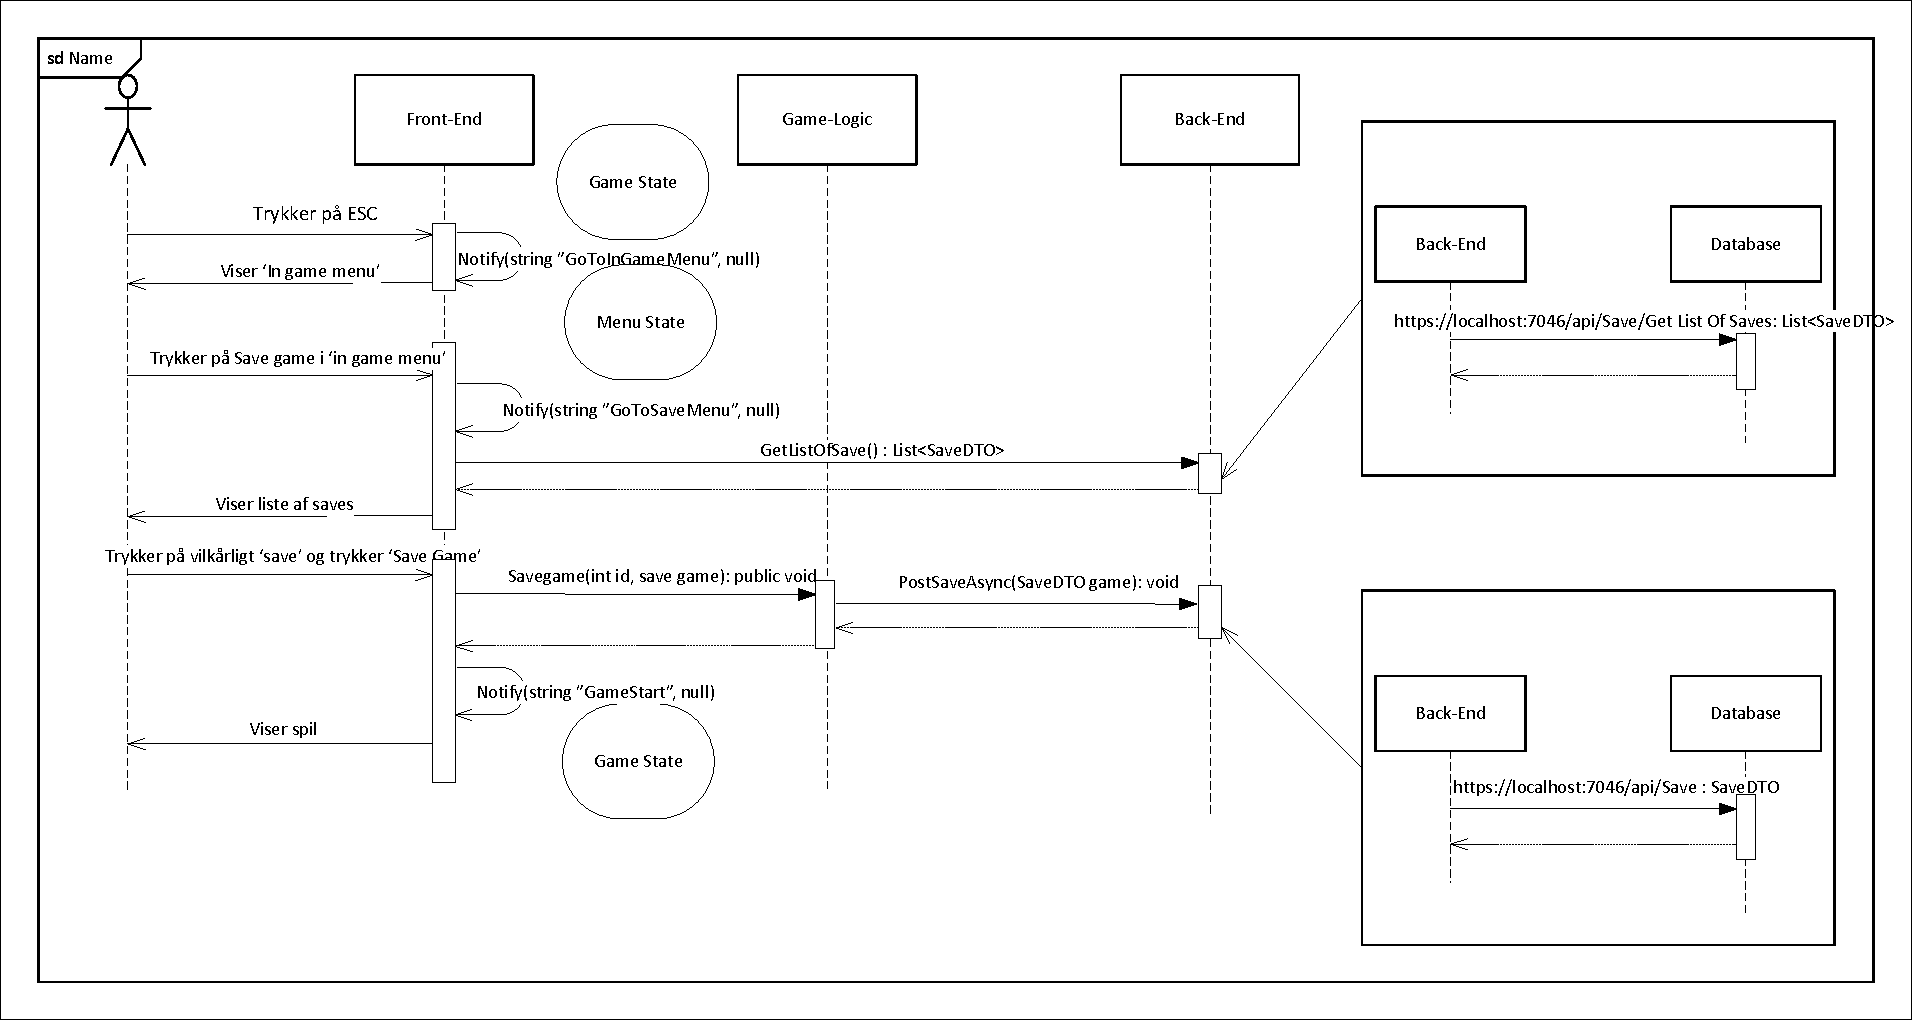
\includegraphics[width = \textwidth]{02-Body/Images/Arkitektur - SD Login}
\caption{SD diagram for User Story 1. Diagrammet viser hvordan systemet overordnet skal kommunikere på tværs når bruger skal logge ind}
\label{fig:Arkitektur-SD-Login}
\end{figure}

\noindent  Herunder ses et sekvensdiagram for User Story 2 - Opret Bruger. Her ses hvordan det ønskes at de forskellige moduler kommunikerer på tværs af systemet når bruger skal oprette en bruger i systemet.
\begin{figure}[H]
\centering
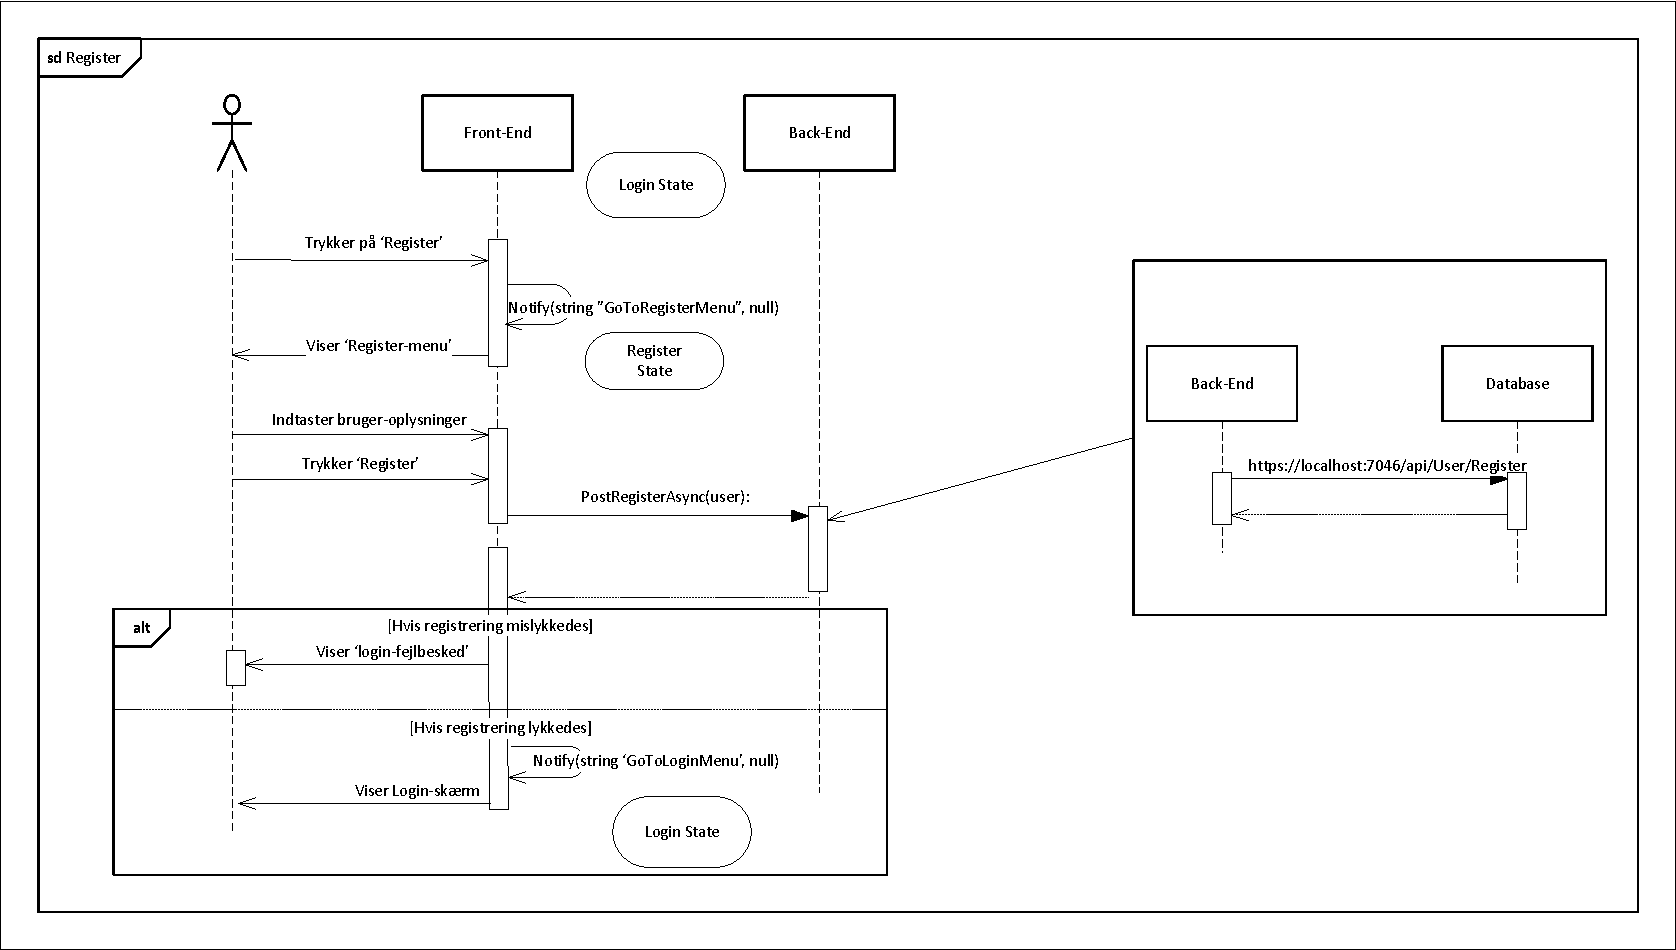
\includegraphics[width = \textwidth]{02-Body/Images/Arkitektur - SD Register}
\caption{SD diagram for User Story 2. Diagrammet viser hvordan systemet overordnet skal kommunikere på tværs når bruger skal oprette en bruger i systemet}
\label{fig:Arkitektur-SD-Register}
\end{figure}

\subsection{Frontend Design}

I frontenden ønskes det at hele spillet foregår i et vindue. Det er derfor nødvendigt at programmet kan skifte mellem forskellige views uden at skulle åbne et nyt vindue, hver gang der skiftes. Løsningen til denne udfordring beskrives nærmere i implementerings afsnittet, nemlig \autoref{sec:Frontend Implementering}.
Spillet vil bestå af en række af vinduer, som giver spilleren den nødvændige information for at de kan spille spillet (så som at logge ind, gemme og hente spil, samt spille spillet).\\
Inden arbejdet på Frontend arkitekturen begyndte, er der blevet lavet en teknologiundersøgelse \autoref{sec:unity-.net}, om hvilket udviklingsværktøj Frontenden og derigennem spillet skulle udvikles i. Baseret på denne teknologiundersøgelse er der blevet valgt, at spillet vil blive udviklet i et .NET framework. Dette valg er blandt andet truffet da dette framework passer bedre med den opdeling af arbejde der er lavet i projektgruppen, altså opdelingen af Frontend og Backend. For andre grunde, se \autoref{sec:unity-.net}, hvor flere fordele og ulemper for både unity og .NET frameworket er sat op.\\
Her følger en række af mockups\footnote{Lavet i Unity} af nogle af spillets views.

\subsubsection{Room}

Room view (\autoref{fig:Design-FE-mockup-room}) er det primære spil-vindue. Her præsenteres spilleren for en beskrivelse af det rum de er i, samt hvilke elementer i rummet de kan interagere med. Der vises også et kort over banen. Kortet Viser kun de rum spilleren allerede har været i, mens resten holdes skjult. Når brugeren så besøger et nyt rum, kan dette ses selvom spilleren forlader rummet. Dette lader spilleren udforske og oplåse hele kortet.\\
En række knapper nederst i højre hjørne på skærmen giver spilleren mulighed for at interagere med spillet. Fire knapper ("Go {North/West/South/East}") lader spilleren gå fra et rum til et andet. Ikke alle rum har forbingelse til alle sider, så det er f.eks. ikke altid muligt at trykke på "Go North". Kortet og rum beskrivelsen fortæller hvilken vej det er muligt at bevæge sig i.\\
Udover de fire retningsknapper er der et antal andre knapper. Disse bruges til at gemme spillet, gå til menuer, samt interagere med elementerne i rummet. Det specifikke antal og deres funktion er afhængig af den præcise implementering.

\begin{figure}[H]
\centering
\includegraphics[width = \textwidth]{02-Body/Images/RoomMockup.PNG}
\caption{Et mockup af det primære spil vindue. Tekst øverst i venstre side af skærmen giver en beskrivelse af det rum spilleren er i, samt en liste af elementer i rummet som spilleren kan interagere med. Øverst til højre vises et billede af banen. Spilleren interagerer med spillet via knapper nederst i højre hjørne. Knapperne "Go {North/West/South/East}" fører spilleren ind i et andet rum, mens de resterende knapper (markeret "Button") bruges til andre funktionaliterer i spillet.}
\label{fig:Design-FE-mockup-room}
\end{figure}

\subsubsection{Combat}

Combat vinduet er baseret på room vinduet. Strukturen er den samme: der er et kort øverst til højre, en beskrivelse øverst til venstre og knapper neders til højre. Nederst til venstre er der information om hvordan kampen går,  i stedet for en liste af elementer i rummet.\\
Knapperne består af nogle "menu" knapper, som lader dig gå til spil menuer, samt en 'Fight' knap og en 'Flee' knap. 'Fight' knappen lader spilleren kæmpe mod fjenden, mens 'Flee' knappen lader spilleren flygte fra kampen og tilbage til rummet som spilleren kom fra.


\begin{figure}[H]
\centering
\includegraphics[width = \textwidth]{02-Body/Images/CombatMockup.PNG}
\caption{Combat view. Spilleren præsenteres for en fjende, og får information om hvordan kampen mod fjenden går. Der er knapper til at kæmpe og flygte, samt gå til menuer. øverst til højre er kortet over banen, ligesom i Room vinduet \autoref{fig:Design-FE-mockup-room}.}
\label{fig:Design-FE-mockup-combat}
\end{figure}


\subsubsection{Login}

Når spillet startes bedes spilleren prompte at logge ind på deres profil. Dette sker i login vinduet. Spilleren kan indtaste sit brugernavn og kodeord i de to tekstfelter 'Username' og 'Password'. Knappen login fører dem videre til spillet, hvis det indtastede login er korrekt.\\
Knappen create user fører spilleren til et vindue som ligner login vinduet, og som lader spilleren oprætte en ny bruger.\\
Exit lukker spillet.

\begin{figure}[H]
\centering
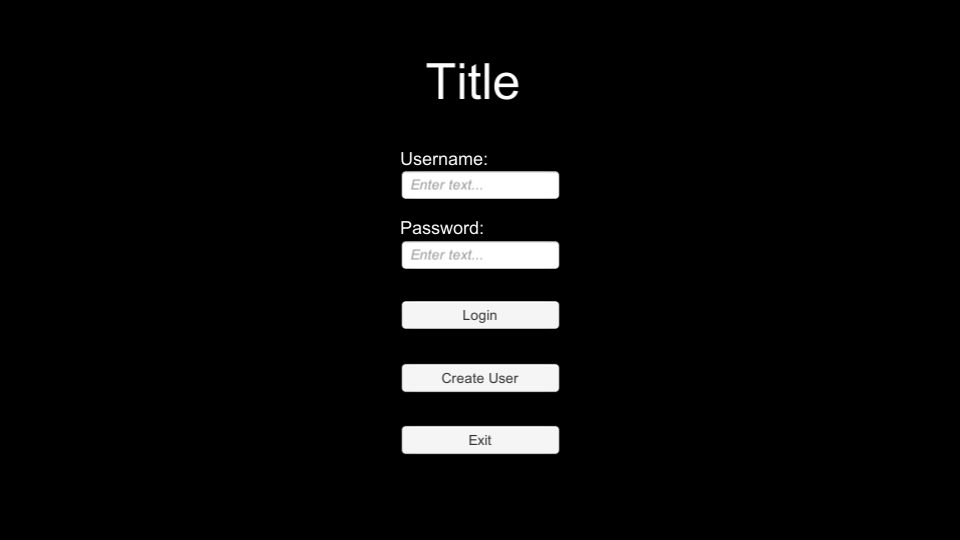
\includegraphics[width = \textwidth]{02-Body/Images/LoginMockup.PNG}
\caption{Login view. Bruger kan indtaste sit brugernavn og kodeord for at få adgang til spillet, eller trykke på create user for at komme til et vindue hvor man kan oprætte en ny bruger. Det er også muligt at forlade spillet igen.}
\label{fig:Design-FE-mockup-login}
\end{figure}

\subsubsection{Settings}
Settings viduet tillader at spilleren kan ændre indstillinger for spillet, og kan tilgås fra hovedmenuen, samt fra selve spillet.\\
Det er her muligt at ændre f.eks. skærmopløsning og lydstyrke. Det er muligt at gemme de indstillinger som er valgt, forlade menuen uden at gemme de valgte indstillinger, samt gendanne standard indstillingerne for spillet. 

\begin{figure}[H]
\centering
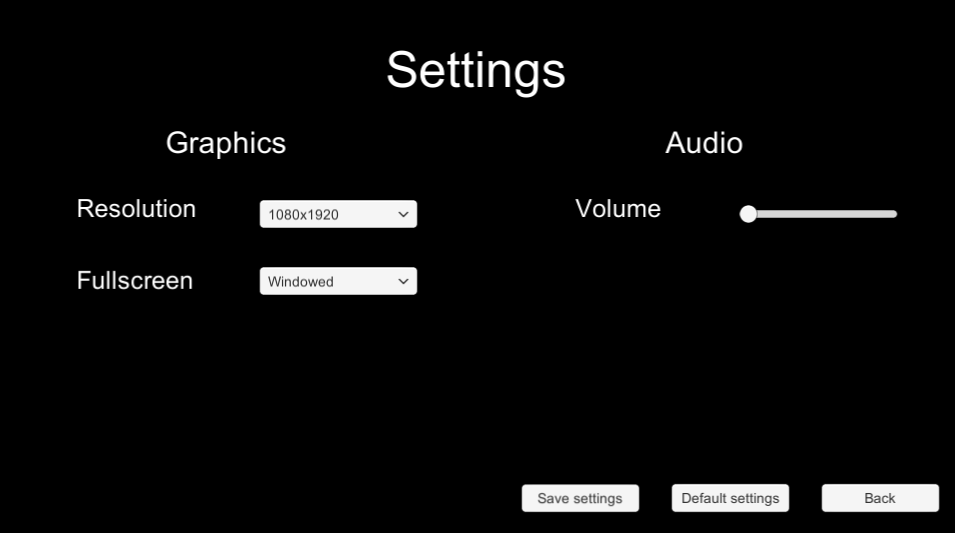
\includegraphics[width = \textwidth]{02-Body/Images/settingsMockup.PNG}
\caption{Settings view. Tillader at man kan ændre indstillinger for spillet, så som skærmopløsning og lydstyrke. Det er muligt at gemme indstillingerne, forlade skærmen uden at gemme indstillingerne, samt sætte spillet tilbage til standard indstilinger.}
\label{fig:Design-FE-mockup-settings}
\end{figure}

\newpage

\subsection{Game Controller Design}
Game Controllerens endelige design følger arkitekturen tæt og tager udgangspunkt i de funktioner som skal kaldes i modulet Front-end. I dette afsnit fokuseres der på de features i spillet som gør spillet funktionelt og giver brugeren et reelt gameplay.

\subsubsection{Map Creation}
Når bruger vælger at starte et spil eller loade et spil fra Front-end siden, skal Game Controlleren indlæse et map så Front End kan fremvise det for bruger. Det ønskes at dette sker ved at Game Controlleren indlæser et tekstdokument(.txt-fil), hvor rummet er repræsenteret med de forskellige veje til et nyt rum. Herfra skal der hentes beskrivelser af de forskellige rum fra databasen via Back-End modulet. Derved når der skiftes rum i Front-end modulet, så sendes beskrivelsen til Front-End modulet som derefter kan vise beskrivelsen for det specifikke rum til brugeren.

\subsubsection{Player class og Items}
\label{sec:Player class og Items}
Heri skal der implementeres stats til spilleren. I vores implementation kommer der to færdigheder som kan have en indflydelse på spillerens forløb under combat. De to færdigheder er HealthPoints og ArmorClass. HealthPoints skal udgøre hvor meget skade spilleren kan tage inden død. ArmorClass skal udgøre hvor højt fjenden skal slå for at give skade til spilleren. Heri skal implementeres items som kan forøge spillerens chancer for at gennemføre de forskellige fjender. Heri vil der være 'shields' som forøger variablen ArmorClass for spilleren, så fjenden skal slå højere for at give skade til spilleren. Den anden type item er våben som er med til at øge spillerens 'terning-rul' for at slå højere end fjendens ArmorClass og skade fjenden. Combat-fasen bliver uddybet yderligere i understående afsnittet \autoref{sec:Combat-design}.

\subsubsection{Enemies}
Fjender skal implementeres på samme måde som spilleren. Deres færdigheder såsom HealthPoints, ArmorClass og Attack(våben)skal dog være forudbestemt. Fjenderne er fordelt over mappet og skal være gradvist stærkere jo længere spilleren kommer i spillet. Dette skal gøres ved at forøge deres færdigheder. Disse fjenders færdigheder og navne skal hentes fra GameControlleren af Front-End, når spillet startes af brugeren. Når bruger så går ind i et givet rum, hvor en fjende er til stede, går spillet ind i combat state. Når fjender er blevet bekæmpet, lagres det i databasen via back-end modulet når bruger vælger at gemme spillet. Når bruger dernæst åbner det gemte spil, er fjenden bekæmpet og fjernet fra spillet.
\subsubsection{Combat}
\label{sec:Combat-design}
Combat skal initieres når spiller går ind i et rum hvor der er en fjende til stede. Spillet vil derefter gå ind i et combat state hvor spilleren får mulighed for at angribe fjenden eller flygte(flee) og gå tilbage til det forrige rum. Nogle af disse combat interaktioner skal være obligatoriske, så spilleren er nødsaget til at færdiggøre combat for at komme videre i spillet. Når der angribes vil der være implementeret to terninger der bestemmer om spilleren rammer og hvor meget spilleren skader fjenden. For fjenden vil der blive implementeret det samme. Spillerens færdigheder vil have en indflydelse på kampens fremgang(Se afsnit \autoref{sec:Player class og Items}). Herefter vil der først blive tjekket om fjenden har mere HealthPoints tilbage og efterfølgende det samme for spilleren. Der vil være to outcomes for combat state. Enten bekæmpes fjenden af spilleren eller vice versa. Når spilleren bekæmper fjenden, vil rummet som spilleren gik ind i, blive tilgængeligt for spilleren. Hvis spilleren bliver bekæmpet af fjenden, vil spillet gå til end-screen, hvor bruger får mulighed for at lukke spillet eller gå til hovedemenu.

\subsubsection{Saves}
Når bruger vil stoppe spillet, vil der blive implementeret en funktion for brugeren at gemme sine fremskridt i spillet. Brugeren kan dermed gemme spillet i menuen som lagre spillets fremskridt i databasen via Back-End Modulet. Herunder vil dataen der bliver sendt, være rum der er blevet besøgt, fjender der er bekæmpet og genstande der er blevet samlet op og udrustet. Når bruger vil åbne det save igen, vil dataen blive sendt tilbage så bruger kan fortsætte med samme fremskridt.
\subsection{Backend Design}
\label{ssec: Backend Design}

I det følgende afsnit beskrives design overvejelser i forbindelse med udviklingen af systemets backend Web Api. Afsnittet vil give et overblik over hvilke resources/routes Web api’et stiller til rådighed. Efterfølgende forklares hvordan Data transfer objects vil blive anvendt, hvordan Authentication og Autherization vil blive håndteret, samt hvordan passwords vil blive hashed. Hertil vil en BackEndController klasse, som skal bruges på client siden blive redegjort for. Tilslut præsenteres applikationsmodeller over controller klasserne for de relevante User Stories, som består af en række sekvens og klasse diagrammer.\\

\subsubsection{Analyse konklusion}
I dette projekt vil give bedst mening at anvende mulighed 1 baggrunden for denne beslutning kan ses i \autoref{ssec: Teknisk Analyse Backend} med en backend bestående af ASP.NET og EF Core. Her fåes nemlig muligheden for at separere data resourcerne fra resten af applikationen samtidig med vi for en mere sikker og pålidelig håndtering af brugere samtidig med EF Core stadig understøttes til kommunikation med databasen i gennem LINQ. \cite{Language Integrated Query}\\


\subsubsection{Routes}
Applikationens nødvendige routes kan inddeles i to under grupper ”Save”, som indeholder routes relateret til game state og ”User”, som indeholder routes relateret til brugeren. Alle routes som omhandler game state skal authorizes, mens routes, som omhandler brugeren tilader anonyme forespørgelser. Nedenfor er givet en oversigt over de forskellige routes med en tilhørende beskrivelse.\\

\textbf{Save:}\\
\begin{itemize}
\item GET: /api/Save
Denne route henter et sepcifikt gemt game state fra databasen, for den bruger som er logget ind.
\item POST: /api/Save\\
Denne route sender et scecifikt game state til databasen, for den bruger som er logget ind.
\item GET: /api/Save/Get List Of Saves\\
Denne route henter en liste af game states, for den bruger som er logget ind. 
\item GET: /api/Save/Get Room Description\\
Denne route henter en beskrivelse af det valgt rum i spillet.
\end{itemize}

\textbf{User:}\\
\begin{itemize}
\item POST: /api/User/Register\\
Denne route registrerer en ny bruger ved at gemme oplysninger om denne i databasen, og returnerer en JWT token. Når en bruger bliver registreret får den tildelt 5 pladser i databasen til game states.
\item POST: /api/User/Login\\
Denne route logger en bruger ind ved at tjekke bruger oplysninger med dem, som er registreret i databasen, denne route returnerer også en JWT token.
\end{itemize}

\subsubsection{Data Transfer Object:}

De data objekter som gemmes i SQL databasen vil indeholde nogle navigational properties, som bruges til at query data’en og til at opretter relationer mellem objekterne. Da disse properties ikke har nogen relevans for clienten oprettes der følgende DTO’er for modellerne User og Save som ses på \autoref{fig:Design-Backend-DTO}\\

\begin{figure}[H]
\centering
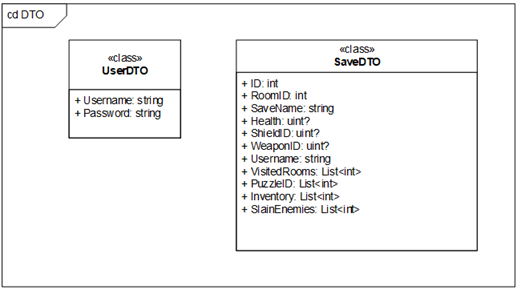
\includegraphics[width = \textwidth]{02-Body/Images/Backend_DTO.PNG}
\caption{klasse diagram over DTO'er for User og Save}
\label{fig:Design-Backend-DTO}
\end{figure}

På den måde kan man sikre at kun den nødvendige data sendes til clienten.\\

\subsubsection{Authentication/Authorization med JWT Token}
JWT (Jason Web Token) er et JSON object, som bruges til at validere (Authenticate), og til at afgøre hvorvidt en client har adgang til den givne data (Authorizing). En token består af tre dele en header, en payload og en signature.\\

\textbf{Header:}\\
Headeren består af en type og en hashing algoritme, typen vil for dette system være ”JWT” og algortimen vil være ”HmacSha256”.\\

\textbf{Payload:}\\

Payloaden indeholder såkaldte claims, der findes tre typer af claims reserved, public og private. Reserved er en række prædefineret claims som kan bruges til eksempelvis at sætte en tidsbegrænsning på den gældende. Public og private claims kan indeholde noget information omkring brugeren. I dette system benyttes private claims til at indeholde brugerens username, som så kan bruges til at genkende hvem den aktuelle token tilhører ved en forespørgsel.\\

\textbf{Signature:}\\
Signature bruges til at verificere hvem som er afsender af JWT’en, og til sikre at den ikke er blevet ændret undervejs. Her samles header, payload og en ”secret” som er en hemmelig string af tegn, kun Web Api'et kender.
For at generere denne token implementeres en funktion, som opretter en token efter de forhold som er beskrevet ovenfor.\\


\subsubsection{Hashing}
\label{sssec: Hashing}
Under design fasen blev det besluttet at anvende hashing til at gemme en brugers password i databasen, for at øge sikkerheden. Sikkerhed var ellers ikke prioteret i vores MoSCoW analyse \autoref{ssec:MOSCOW}, for denne udgave af spillet.
Hashing af passwords går ud på at kryptere det gemte password i databasen. Det skal krypteres således at det ikke er muligt at dekryptere, samtidig med at det stadig kan valideres om det er et korrekt password, der modtages af en client. Når et password hashes anvendes et såkaldt ”salt”, som er en tilfældigt genereret string kobineret med password’et.\\

Til at Hashe passwords med anvendes Bcrypt \cite{Bcrypt}, dette library stiller hashing af passwords til rådighed. Der findes en C\# udgave kaldet Bcrypt.Net  som vil blive anvendt. Helt præcist er det funktionen HashPassword(”password”, BcryptWorkfactor), denne funktion skal have en BcryptWorkfactor, hvilket er et tal der siger noget om hvor mange iterationer Bcrypt vil bruge på at generere det ”salt” til at hashe password’et med. Her anbefales det at bruge en værdi på 11, da det generelt set anses som tilstrækeligt niveau hvad angår sikkerhed.
Funktionen verify(”password”, hashedpassword) bruges til at verificere om et givent password svare til dets krypterede udgave.\\

\subsubsection{BackEndController på client siden}
Til brug af clienten for at tilgå backenden, skal der bruges en BackendController klasse, dennes ansvar vil være at udføre HTTP request/responses, og vil indeholde en funktion for hvert endpoint.\\
 
Klassen vil gøre brug af en HttpClient som er en klasse .Net stiller til rådighed til at håndtere HTTP request/responses. Da backenden kræver en JWT for at få adgang til endpoints, hvad angår loading og saving af game state, skal clienten også gemme JWT for den bruger som er logget ind, således at den kan blive sendt med de forskellige requests.


\subsection{Applikationsmodeller}
I dette afsnit gennemgåes applikationsmodeller for de enkelte user stories, der udarbejdes sekvensdiagrammer for at beskrive funktionalitet og klasse diagrammer til at beskrive indeholdet og sammen spillet imellem klasserne. Applikationsmodellerne deles op efter controllere, en for UserControlleren og en for SaveControlleren. Fokuset vil her ligge på controller klasserne, for en beskrivelse af DAL komponenterne henvises til database design afsnitet \autoref{ssec:DB Design}.\\

\subsubsection{Applikationsmodel User Controller}
\textbf{User Story 1: Log in}\\
Når clienten udfører en HTTP request med URL’en : ” https://localhost:7046/api/User/Login”, udføres følgende aktioner som fremgår af sekvensdiagrammet på \autoref{fig:Design-Backend-Sekvens-1}\\ 

\begin{figure}[H]
\centering
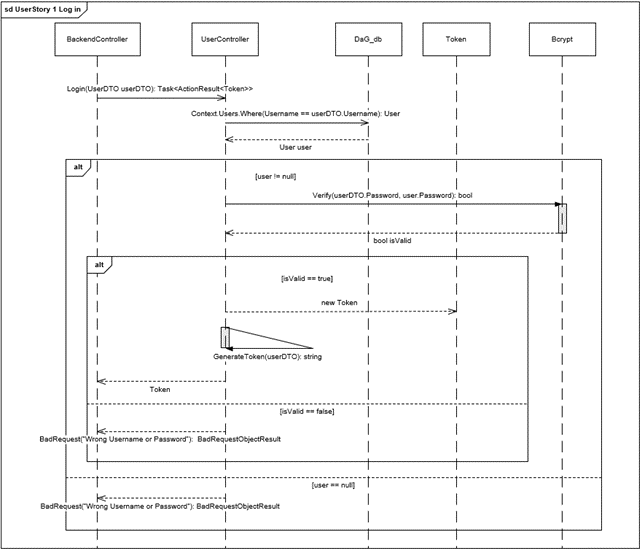
\includegraphics[width = \textwidth]{02-Body/Images/Backend_sekvens_1.PNG}
\caption{Sekvensdiagram som viser funktionaliteten i User Story 1 Log in}
\label{fig:Design-Backend-Sekvens-1}
\end{figure}

Authentication controlleren fra C3 modellen hedder her “UserController” og har til opgave at gøre det muligt for en bruger at registrere sig og logge ind. Login implementeres i Login() funktionen, som er det endpoint clienten kalder for at logge ind. Her bliver der tjekket om det indtastede brugernavn findes i databasen. Hvis brugernavnet findes, så bliver adgangskoden tjekket med funktionen verify fra Bcrypt klassen, og passer den, bliver der returneret en JWT token. Hvis brugernavnet derimod allerede eksiterer eller adgangskoden ikke er korrekt retuneres en fejlmeddelse.\\

\textbf{User Story 2: Opret Bruger}\\
Når clienten udfører en HTTP request med URL’en : ” https://localhost:7046/api/User/Register”, udføres følgende aktioner som fremgår af sekvensdiagrammet på \autoref{fig:Design-Backend-Sekvens-2}\\

\begin{figure}[H]
\centering
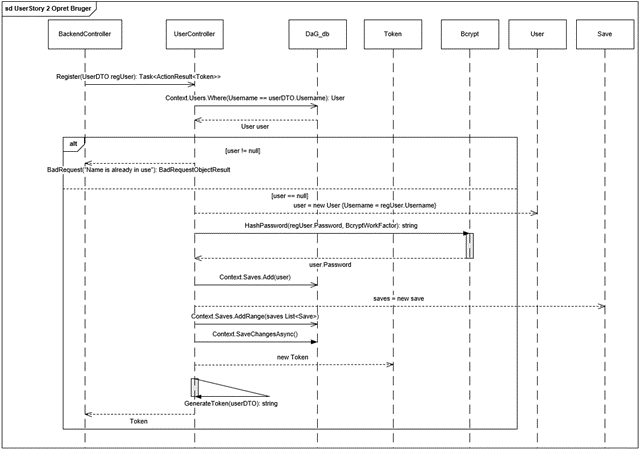
\includegraphics[width = \textwidth]{02-Body/Images/Backend_sekvens_2.PNG}
\caption{Sekvensdiagram som viser funktionaliteten i User Story 2 Opret Bruger}
\label{fig:Design-Backend-Sekvens-2}
\end{figure}

For at kunne logge ind skal det være muligt at oprette en bruger til dette laves en Register(UserDTO regUser) funktion. Denne starter med at checke om brugernavnet er optaget. Er den det, returneres der en fejlmeddelelse, og ellers registreres brugeren. Dernæst bliver det valgte kodeord ”hashed”, således at der opnås en vis sikkerhed i systemet. Når der oprettes en ny bruger skal denne have tildelt 5 pladser i databasen til sine gemte spil, dette sker ved at der oprettes en liste af saves der indeholder 5 nye saves, disse gemmes med contexten i SQL databasen. Hvis alt går godt retuneres en JWT token.\\

\textbf{Samlet Klasse diagram over User Story 1 og 2}\\

På \autoref{fig:Design-Backend-Klasse-1-2} kan ses en oversigt over de klasser, metoder og attributter, som anvendes i udførelsen af User story 1 og 2. Hertil anvendes også klassen Bcrypt som ikke er taget med, da den blot er brugt udefra, detaljer om Bcrypt kan ses i afsnitet ovenover \autoref{sssec: Hashing}.\\

\begin{figure}[H]
\centering
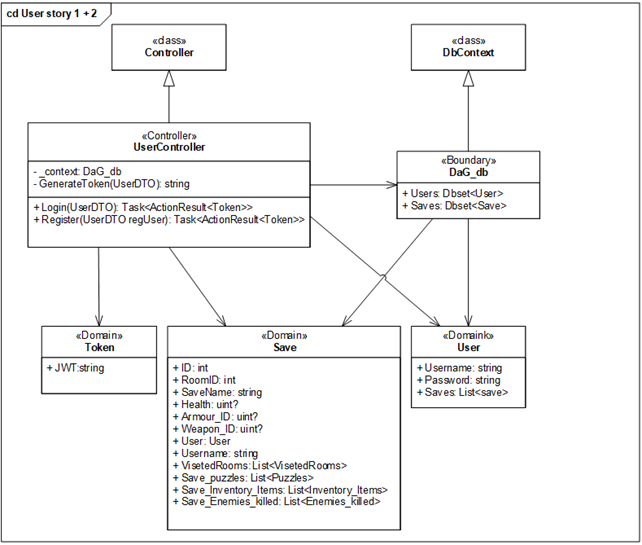
\includegraphics[width = \textwidth]{02-Body/Images/Backend_klasse_1_2.PNG}
\caption{Samlet klasse diagram over User story 1 og 2}
\label{fig:Design-Backend-Klasse-1-2}
\end{figure}

\subsubsection{Applikationsmodel Save Controller}
\textbf{User Story 7: Exit Menu -\g Save and Exit}\\
Load/save controlleren fra C3 modellen er blevet til en enkelt controller, som kaldes for ”SaveController”. Denne controller har til ansvar at gemme et spil, men samtidig også være i stand til at kunne hente gemte spil, altså at loade dem.
Når clienten udfører en HTTP request med URL’en : ” https://localhost:7046/api/Save”, udføres følgende aktioner som fremgår af sekvensdiagrammet på \autoref{fig:Design-Backend-Sekvens-7}\\

\begin{figure}[H]
\centering
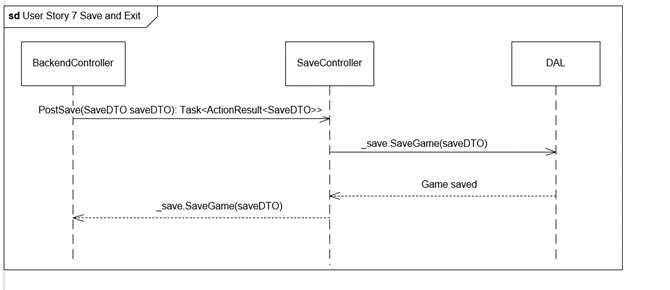
\includegraphics[width = \textwidth]{02-Body/Images/Backend_sekvens_7.PNG}
\caption{sekvensdiagram over User Story 7 Save and Exit}
\label{fig:Design-Backend-Sekvens-7}
\end{figure}

Der bruges en httpPost funktion kaldet PostSave som gemmer et nyt spil i databasen ved at ligge det modtagene gamestate fra parameter listen ind i et funktionskald SaveGame() i DAL klassen, som så sørger for at gemme spillet i databasen på den korrekte måde.\\

\textbf{User Story 17: Exit Menu -\g Save and Exit}\\

Når clienten udfører en HTTP request med URL’en : ” https://localhost:7046/api/Save/Get List Of Saves”, udføres følgende aktioner som fremgår af sekvensdiagrammet på \autoref{fig:Design-Backend-Sekvens-17}\\

\begin{figure}[H]
\centering
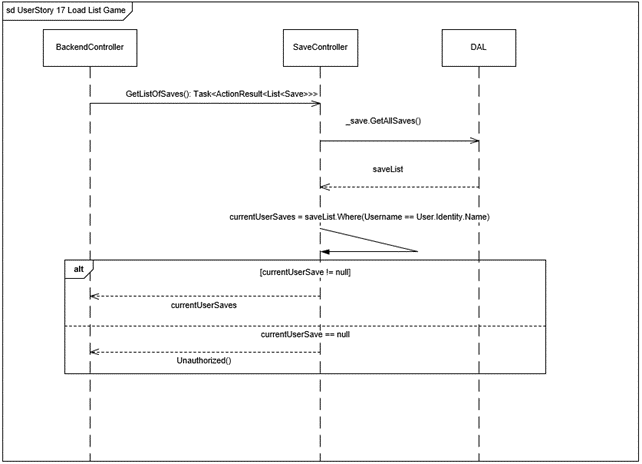
\includegraphics[width = \textwidth]{02-Body/Images/Backend_sekvens_17.PNG}
\caption{Sekvensdiagram over User Story 17 Main Menu -\g Load List Game}
\label{fig:Design-Backend-Sekvens-17}
\end{figure}

Da vi gerne vil gøre det muligt at have 5 save games pr. profil, skal det naturligvis være muligt at kunne vælge mellem de forskellige saves, til dette laves funktion GetListOfSaves(). Clienten kalder her GetListOfSaves() som er et HttpGet endpoint, denne funktion henter alle saves i DAL klassen ved at kalde GetAllSaves(). SaveController finder så de gemte spil i listen hvor brugernavnet passer med den burger, som er logget ind ved brug af User.Identity som stilles til rådighed af ControllerBase klassen, her i kan claims for den nuværende JWT nemlig findes.\\

\textbf{UserStory 18 : Main Menu -\g Load Game -\g Load}\\
Når clienten udfører en HTTP request med URL’en :” https://localhost:7046/api/Save?id={id}”, udføres følgende aktioner som fremgår af sekvensdiagrammet på \autoref{fig:Design-Backend-Sekvens-18}\\

\begin{figure}[H]
\centering
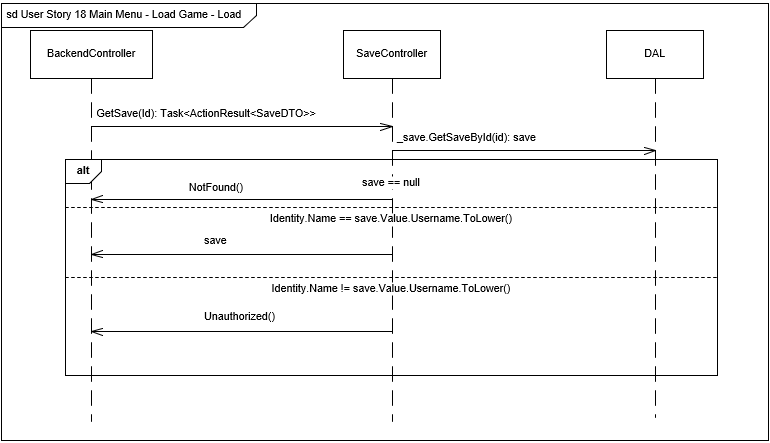
\includegraphics[width = \textwidth]{02-Body/Images/Backend_sekvens_18.PNG}
\caption{Sekvens diagram over User story 18 Main Menu -> Load Game -> Load}
\label{fig:Design-Backend-Sekvens-18}
\end{figure}

\textbf{User Story 19 : Main Menu -\g Load Game -\g Delete Game}\\

Under design fasen blev det besluttet at overskrive gemte saves fremfor at slette og lave et nyt, da et saves Id på den måde ikke ændret sig i databasen når man lavede et nyt save. Derfor er User story 19 som omhandler Delete game ikke taget med i design fasen.\\

\textbf{Samlet klasse diagram over User story 7, 17 og 18}\\
Et Samlet klasse diagram for User story 7, 17 og 18 kan ses på \autoref{fig:Design-Backend-Sekvens-7-17-18}\\

\begin{figure}[H]
\centering
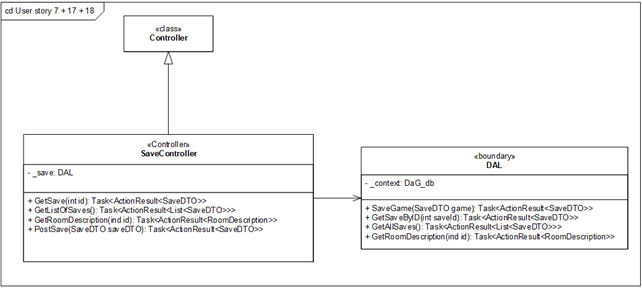
\includegraphics[width = \textwidth]{02-Body/Images/Backend_klasse_7_17_18.PNG}
\caption{Samlet klasse diagram for User story 7, 17 og 18}
\label{fig:Design-Backend-Sekvens-7-17-18}
\end{figure}

Udover de funktioner som bliver brugt i User stories, tilføjes der er en funktion GetRoomDescription, som blot henter en beskrivelse af det rum brugeren befinder sig i.\\


\subsubsection{Konklusion}

Backenden er blevet designet såldedes at den kan håndtere alle de nødvendige kald for at opfylde user stories omkring brugere og gemte spil, dette er beskrevet igennem appilationsmodeller. JWT tokens anvendes til Authentication og Authorization. Til hashing af passwords anvendes Bcrypt. Hertil er BackendControlleren klassen blevet introduceret på clienten, som står for HTTP request/response.\\ 


\newpage

Software Design:
DAL Design
På figur xxx herunder ses klassediagrammet over backend DAL, som benyttes til database access.
Som det kan ses på diagrammet, indeholder DAL en database context, som benyttes til at forbinde backend applicationen til databasen. Derudover består DAL af fire overordnede funktioner, hvoraf de 3 tilhører en user story. Den sidste benyttes når vi starter spillet, til at lave rumbeskrivelser. 


DbClassDiagram.	
 
Følgende funktion benyttes når spil klienten startes, da beskrivelser af rum ikke ændre sig gennem spillets levetid, i den nuværende itteration.
Navn: GetRoomDescription
Parametre: int RoomDescription id
Returtype: Task<ActionResult<RoomDescription>>
Beskrivelse: Denne funktion finder og returnerer en beskrivelse for det valgte RoomDescriptionID. Dette kan også ses på sekvensdiagrammet på figur xxx herunder.
 
User story funktioner
De følgende 3 funktioner benyttes til udførelse af forskellige user stories.
Det drejer sig om:
•	User story 7 – Save game
•	User story 17 – Load game list
•	User story 18 – Load game
Den første funktion SaveGame benyttes til at udføre user story 7.
Her skal der gemmes et spil. Da vi har et krav om kun at holde 5 gemte spil pr bruger, vælger vi, når vi opretter en bruger, at give ham 5 ”tomme” saves. Når brugeren så ønsker at gemme et spil, skal vi ikke tilføje et nyt, men blot overskrive et valgt gammelt save.
Dette kan også ses på sekvensdiagrammet på figur xxx.
Navn: SaveGame
Parametre: SaveDTO
Returtype: Task<ActionResult<SaveDTO>>
Beskrivelse: Da der i vores frontend sørges for at en bruger blot kan have 5 saves, starter vi med at finde det save vi gerne vil overskrive. Det gamle save, samt tilhørende lister slettes, hvorefter det nye save gemmes og eventuelle nye lister til fx. items gemmes.

 
 


 
Den anden funktion GetAllSaves benyttes til at udføre user story 17.
Her skal der loades en liste af gemte spil, når brugeren ønsker at se sine gemte spil. Dette kan også ses på sekvensdiagrammet på figur xxx.
Navn:  GetAllSaves
Parametre: ingen
Returtype: Task<ActionResult<List<Save>>> 
Beskrivelse: Her hentes all gemte saves i spillet.

  

Den tredje funktion GetById benyttes til at udføre user story 18.
Her skal der loades et gemt spil, som brugeren nu ønsker at spille. 
Dette kan også ses på sekvensdiagrammet på figur xxx.
Navn: GetSaveById 
Parametre: int saveID
Returtype: Task<ActionResult<SaveDTO>>
Beskrivelse: Denne funktion finder det save med det medsendte ID, samt tilhørende lister, indsætter værdier i et SaveDTO objekt, hvorefter det returneres. 

 
 

\subsection{Database Design}

Projektets database har gruppen valgt at hoste i lokal storage. Dette er valgt da der under semesterets forløbet opstod problemer med skolens licens af Microsoft produkter. For at undgå at komme ud for udfordringer med hosting senere i forløbet, blev der valgt at gå med den sikre løsning, at hoste databasen lokalt på enheden. Til dette benyttede gruppen et docker image, specifikt det samme image som blev benyttet i DAB undervisning, til vores SQL server.
%(https://docs.microsoft.com/en-us/sql/linux/quickstart-install-connect-docker?view=sql-server-ver15&preserve-view=true&pivots=cs1-powershell)
Hvis ikke der var problemer microsoft, havde gruppen i stedet valgt at lagre data på en cloud-based storage fremfor lokal storage.\\



For at kunne udarbejde et ER diagram til modellering af vores sql database skal vi start med at finde ud af hvilke krav vi har til og hvilke attributter vi ønsker at gemme i vores database.
Først og fremmest ønskede grupper at vi kunne gemme beskrivelserne af de forskellige rum, i spillets layout, for at formindske antallet af filer i klienten, og samtidigt gøre eventuelle senere tilføjelser nemmere.\\ 
Her benyttes rummets id som key, da vi ikke ønsker at man skal kunne oprette flere beskrivelser til samme rum. Diagrammet kan ses på \autoref{fig:ER-Roomdescription}.

\begin{figure}[H]
\centering
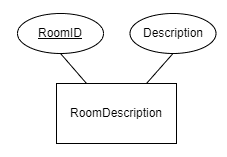
\includegraphics[width = 0.4\textwidth]{02-Body/Images/ER-RoomDescription.PNG}
\caption{ER diagram for Roomdescription. En beskrivelse består blot af en beskrivende string samt det tilhørende unikke rumid.}
\label{fig:ER-Roomdescription}
\end{figure}

Her efter kommer kravene til at kunne gemme et spil for en bruger. Her ønskede vi at man kunne stå et vilkårligt sted i spillet, med untagelse af en combat, og gemme spillet. Det skulle derefter være muligt for spilleren at loade spillet igen, hvorefter spillet er i samme stadie som man gemte det i.
ER diagrammet for at gemme et spil til en bruger på \autoref{fig:ER-GameSave}.
\begin{figure}[H]
\centering
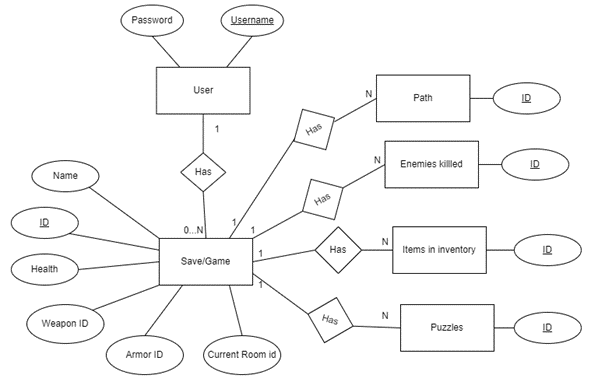
\includegraphics[width = \textwidth]{02-Body/Images/ER-GameSave.PNG}
\caption{ER Diagram til at gemme et spil til en specifik bruger. Her ses de forskellige informationer som skal til for at kunne gemme et helt spil}
\label{fig:ER-GameSave}
\end{figure}

Først og fremmest ønskede gruppen et bruger system, så eventuelle gemte spil kun tilhørte en bruger.
Der gemmes derfor en bruger entitet med et unikt brugernavn og et tilhørende password.
Sikkerhed på password og versalfølsomhed på brugernavnet håndteres af spillets backend.\\
En spiller skal derefter kunne gemme unikke 5 spil med forskellige oplysninger.
Restriktionen med max 5 forskellige spil pr. Bruger, håndteres ved at oprette 5 "tomme" gemte spil ved oprettelsen af en bruger.
Et af disse gemte spil overskriver derfor når vi gemmer. Der kan på denne måde ikke oprettes mere en 5 gemte spil pr. bruger.\\
I et gemt spil ønkede vi at gemme en række forskellige attributter for spilleren.
Første og fremmest får hver spil et unikt id som vi benytter til identifikation og at lave forhold mellem de forskellige tabeller.
Et gemt spil får et navn, valgt af brugeren, som gør det nemmere for brugeren at differentiere mellem de forskellige spil. \\ Dette navn skal være forskelligt fra de 4 andre gemte spil som tilhører samme bruger.\\
En spiller Health gemmes også, da man kan have taget skade efter en kamp.\\
Det gemmes også hvilket rum, spilleren står i når spillet gemmes, så vi loader korrekt tilbage. 
En spiller kan derudover også holde genstande, som armor og våben, i hånden eller i sit inventory. Dette gemmes også henholdsvist som en del af et spil og i en inventory liste tilhørende spillet. 

Tabellen med inventory har 2 atributter, et ID, som svarer til en bestemt genstand, og en reference til set SaveID. Denne parring er unik, da man ikke kan holde 2 af den samme genstand.\\
Tabellerne med Enemies og puzzles fungerer på samme måde. Her har hver enemy og puzzle i spillet et unikt id. Id’et gemmes i kombination med et saveId, som et unikt par, da man ikke kan vinde over samme enimy og løse samme puzzle flere gange.\\
Til slut ønskede vi at kunne vise spilleren de rum som allerede er blevet besøgt. Derfor gemmes der i path tabellen, for hvert spil, en unik kombination af saveID og besøgte rum id. Denne parring er unik da man blot behøver at besøge et rum en gang, før det er synligt på kortet. 

Der er i projektet oprettet klasser tilsvarende ER diagrammerne.
Forholdene mellem disse, samt keys, er opsat i DaG-db klassen og er skrevetved hjælp af fluentAPI. Dette kan ses i Implementationsafsnittet \autoref{Section: DB-Implementering}.

